% CS631 Advanced Programming in the UNIX Environment
% Author: Jan Schaumann <jschauma@netmeister.org>
% $Id: slides.tex,v 1.5 2004/08/04 03:03:44 jschauma Exp $

\documentclass[xga]{xdvislides}
\usepackage[landscape]{geometry}
\usepackage{graphics}
\usepackage{graphicx}
\usepackage{colordvi}

\begin{document}
\setfontphv

%%% Headers and footers
\lhead{\slidetitle}
\chead{CS631 - Advanced Programming in the UNIX Environment}
\rhead{Slide \thepage}
\lfoot{\Gray{Lecture 07: Interprocess Communication}}
\cfoot{\relax}
\rfoot{\Gray{\today}}

\vspace*{\fill}
\begin{center}
	\Hugesize
		CS631 - Advanced Programming in the UNIX Environment\\
		%\vspace{.1in}\includegraphics[scale=0.5]{pics/j1.eps} \\
		Interprocess Communication \\
	\hspace*{5mm}\blueline\\ [1em]

	\Normalsize
		Department of Computer Science\\
		Stevens Institute of Technology\\
		Jan Schaumann\\
		\verb+jschauma@cs.stevens.edu+\\
		\verb+https://www.cs.stevens.edu/~jschauma/631/+
\end{center}
\vspace*{\fill}


\subsection{Pipes: {\tt pipe(2)}}
\small
\setlength{\unitlength}{1mm}
\begin{center}
	\begin{picture}(150,22)
		\thinlines
		\put(0,0){\framebox(130,22){}}
		\put(10,17){{\tt \#include <unistd.h>}}
		\put(10,10){{\tt int pipe(int {\em filedes[2]});}}
		\put(80,3){Returns: 0 if OK, -1 otherwise}
	\end{picture}
\end{center}
\Normalsize
\begin{itemize}
	\item oldest and most common form of UNIX IPC
	\item half-duplex (on some versions full-duplex)
\end{itemize}

\subsection{Pipes: {\tt pipe(2)}}
\begin{center}
	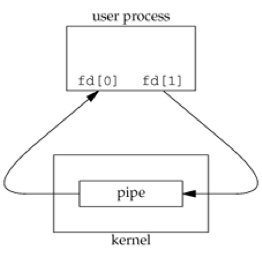
\includegraphics[angle=-90,scale=0.8]{pics/pipe1.eps}
\end{center}

\subsection{Pipes: {\tt pipe(2)}}
\begin{center}
	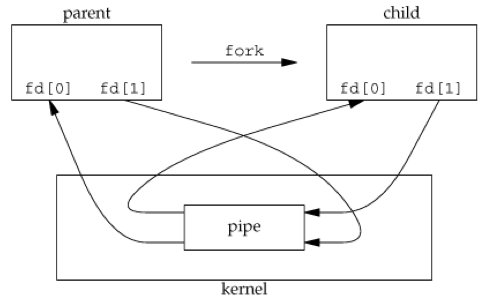
\includegraphics[angle=-90,scale=0.8]{pics/pipe2.eps}
\end{center}

\subsection{Pipes: {\tt pipe(2)}}
\begin{center}
	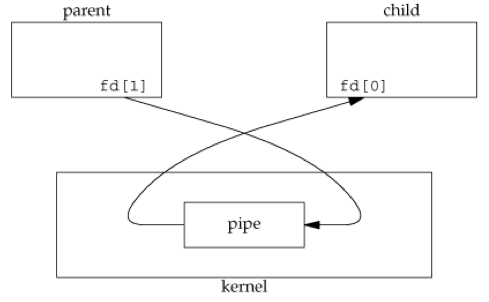
\includegraphics[angle=-90,scale=0.8]{pics/pipe3.eps}
\end{center}

\subsection{Pipes: {\tt pipe(2)}}
\begin{verbatim}
$ cc -Wall pipe1.c
$ ./a.out
P=> Parent process with pid 23988 (and its ppid 7474).
P=> Sending a message to the child process (pid 23989):
C=> Child process with pid 23989 (and its ppid 23988).
C=> Reading a message from the parent (pid 23988):
Hello child!  I'm your parent pid 23988!
$
\end{verbatim}
\vfill
%\hfill \includegraphics[scale=0.9]{pics/j2.eps}


\subsection{Pipes: {\tt pipe(2)}}
\begin{verbatim}
$ cc -Wall pipe1.c
$ ./a.out
P=> Parent process with pid 23984 (and its ppid 7474).
P=> Sending a message to the child process (pid 23985):
C=> Child process with pid 23985 (and its ppid 1).
C=> Reading a message from the parent (pid 1):
Hello child!  I'm your parent pid 23984!
$
\end{verbatim}
\vfill

\subsection{Pipes: {\tt pipe(2)}}
\begin{verbatim}
$ cc -Wall pipe1.c
$ ./a.out
P=> Parent process with pid 23986 (and its ppid 7474).
P=> Sending a message to the child process (pid 23987):
C=> Child process with pid 23987 (and its ppid 23986).
C=> Reading a message from the parent (pid 1):
Hello child!  I'm your parent pid 23986!
$
\end{verbatim}
\vfill

\subsection{Pipes: {\tt pipe(2)}}
A more useful example: displaying some content using the user's preferred
pager.  (Look, Ma, no temporary files!)
\begin{verbatim}
$ cat pipe2.c | ${PAGER:-/usr/bin/more}
$ cc -Wall pipe2.c
$ echo $PAGER

$ ./a.out pipe2.c
[...]
^Z
$ ps -o pid,ppid,command
  PID  PPID COMMAND
22306 26650 ./a.out pipe2.c
22307 22306 more
23198 26650 ps -o pid,ppid,command
26650 26641 -ksh
$ fg
$ env PAGER=/bin/cat ./a.out pipe2.c
\end{verbatim}


\subsection{Pipes: {\tt pipe(2)}}
\small
\setlength{\unitlength}{1mm}
\begin{center}
	\begin{picture}(150,22)
		\thinlines
		\put(0,0){\framebox(130,22){}}
		\put(10,17){{\tt \#include <unistd.h>}}
		\put(10,10){{\tt int pipe(int {\em filedes[2]});}}
		\put(80,3){Returns: 0 if OK, -1 otherwise}
	\end{picture}
\end{center}
\Normalsize
\begin{itemize}
	\item oldest and most common form of UNIX IPC
	\item half-duplex (on some versions full-duplex)
	\item can only be used between processes that have a common ancestor
	\item can have multiple readers/writers ({\tt PIPE\_BUF} bytes are
		guaranteed to not be interleaved)
\end{itemize}
\vspace{.5in}

Behavior after closing one end:
\begin{itemize}
	\item {\tt read(2)} from a pipe whose write end has been closed returns 0
		after all data has been read
	\item {\tt write(2)} to a pipe whose read end has been closed generates
		{\tt SIGPIPE} signal.  If caught or ignored, {\tt write(2)} returns an
		error and sets {\tt errno} to {\tt EPIPE}.
\end{itemize}

\subsection{Pipes: {\tt popen(3)} and {\tt pclose(3)}}
\small
\setlength{\unitlength}{1mm}
\begin{center}
	\begin{picture}(150,40)
		\thinlines
		\put(0,0){\framebox(130,40){}}
		\put(10,35){{\tt \#include <stdio.h>}}
		\put(10,28){{\tt FILE *popen(const char *{\em cmd}, const char *{\em type});}}
		\put(62,21){Returns: file pointer if OK, {\tt NULL} otherwise}
		\put(10,10){{\tt int pclose(FILE *{\em fp});}}
		\put(55,3){Returns: termination status {\em cmd} or -1 on error}
	\end{picture}
\end{center}
\Normalsize
\vspace{.5in}
\begin{itemize}
	\item historically implemented using unidirectional pipe (nowadays
		frequently implemented using sockets or full-duplex pipes)
	\item {\em type} one of ``r'' or ``w'' (or ``r+'' for
		bi-directional communication, if available)
	\item {\em cmd} passed to {\tt /bin/sh -c}
\end{itemize}

\subsection{Pipes: {\tt popen(3)} and {\tt pclose(3)}}
\begin{verbatim}
$ cc -Wall popen.c
$ echo $PAGER

$ ./a.out popen.c
[...]
$ env PAGER=/bin/cat ./a.out popen.c
[...]
$
\end{verbatim}
\vfill
%\hfill \includegraphics[angle=-90,scale=0.9]{pics/j3.eps}

\subsection{Pipes: {\tt popen(3)} and {\tt pclose(3)}}
\begin{verbatim}
$ cc -Wall popen.c
$ echo $PAGER

$ ./a.out popen.c
[...]
$ env PAGER=/bin/cat ./a.out popen.c
[...]
$ env PAGER=/bin/cat/foo ./a.out popen.c
sh: /bin/cat/foo: Not a directory
$ env PAGER="more; touch /tmp/boo" ./a.out popen.c
$ env PAGER="more; rm /etc/passwd 2>/dev/null" ./a.out popen.c
\end{verbatim}
\vfill
%\hfill \includegraphics[scale=0.9]{pics/j4.eps}


\subsection{FIFOs: {\tt mkfifo(2)}}
\small
\setlength{\unitlength}{1mm}
\begin{center}
	\begin{picture}(150,22)
		\thinlines
		\put(0,0){\framebox(130,22){}}
		\put(10,17){{\tt \#include <sys/stat.h>}}
		\put(10,10){{\tt int mkfifo(const char *{\em path}, mode\_t {\em mode});}}
		\put(80,3){Returns: 0 if OK, -1 otherwise}
	\end{picture}
\end{center}
\Normalsize

\begin{itemize}
	\item aka ``named pipes''
	\item allows unrelated processes to communicate
	\item just a type of file -- test for using {\tt S\_ISFIFO(st\_mode)}
	\item {\em mode} same as for {\tt open(2)}
	\item use regular I/O operations (ie {\tt open(2)}, {\tt read(2)}, {\tt
		write(2)}, {\tt unlink(2)} etc.)
	\item used by shell commands to pass data from one shell
			pipeline to another without creating intermediate
			temporary files
\end{itemize}

\subsection{FIFOs: {\tt mkfifo(2)}}
Example: split input into sets
\begin{center}
	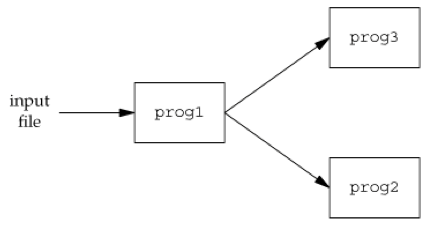
\includegraphics[angle=-90,scale=0.8]{pics/fifo1.eps}
\end{center}

\subsection{FIFOs: {\tt mkfifo(2)}}
Example: split input into sets
\begin{center}
	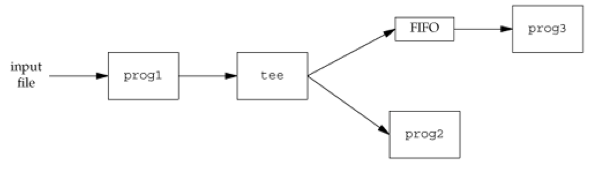
\includegraphics[angle=-90,scale=0.8]{pics/fifo2.eps}
\end{center}
\begin{verbatim}
$ mkfifo fifo
$ grep pattern fifo > match &
$ gzcat file.gz | tee fifo | grep -v pattern > nomatch
\end{verbatim}
\vfill
%\hfill \includegraphics[scale=0.9]{pics/j5.eps}

\subsection{System V IPC}
Three types of IPC originating from System V:
\begin{itemize}
	\item Semaphores
	\item Shared Memory
	\item Message Queues
\end{itemize}
\vspace{.5in}

All three use {\em IPC structures}, referred to by an {\em identifier} and a
{\em key}; all three are (necessarily) limited to communication between
processes on one and the same host.
\\

Since these structures are not known by name, special system calls ({\tt
msgget(2)}, {\tt semop(2)}, {\tt shmat(2)}, etc.) and special userland
commands ({\tt ipcrm(1)}, {\tt ipcs(1)}, etc.) are necessary.


\subsection{System V IPC: Semaphores}
A semaphore is a counter used to provide access to a shared data object for
multiple processes.  To obtain a shared resource a process needs to do the
following: \\

\begin{enumerate}
	\item Test semaphore that controls the resource.
	\item If value of semaphore $>$ 0, decrement semaphore and use resource;
		increment semaphore when done
	\item If value == 0 sleep until value $>$ 0
\end{enumerate}
\vspace{.5in}
Semaphores are obtained using {\tt semget(2)}, properties controlled using
{\tt semctl(2)}, operations on a semaphore performed using {\tt semop(2)}.

\subsection{System V IPC: Semaphores}
\begin{verbatim}
$ cc -Wall semdemo.c
1$ ./a.out

2$ ./a.out

$ ipcs -s
\end{verbatim}

\subsection{IPC data flow}
\begin{center}
	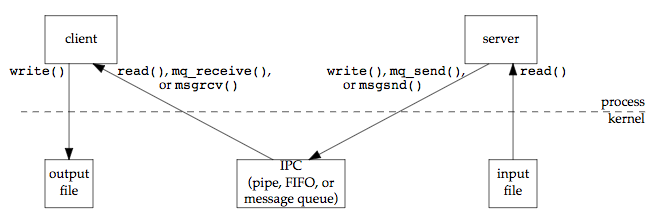
\includegraphics[angle=-90,scale=0.8]{pics/ipcflow.eps}
\end{center}

\subsection{System V IPC: Shared Memory}

\begin{center}
	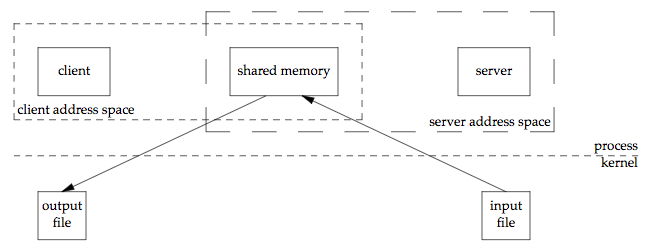
\includegraphics[angle=-90,scale=0.8]{pics/shmflow.eps}
\end{center}



\subsection{System V IPC: Shared Memory}
\begin{itemize}
	\item fastest form of IPC
	\item access to shared region of memory often controlled using
		semaphores
	\item obtain a shared memory identifier using {\tt shmget(2)}
	\item catchall for shared memory operations: {\tt shmctl(2)}
	\item attach shared memory segment to a processes address space by
		calling {\tt shmat(2)}
	\item detach it using {\tt shmdt(2)}
\end{itemize}

\subsection{System V IPC: Shared Memory}
\begin{verbatim}
$ cc -Wall shmdemo.c
$ ./a.out "Cow says: 'Moo!'"
$ ./a.out
$ ipcs -m
\end{verbatim}

\subsection{System V IPC: Shared Memory}
\begin{verbatim}
$ cc -Wall memory-layout.c
$ ./a.out
array[] from 804a080 to 8053cc0
stack around bffff9e4
malloced from 8053cc8 to 806c368
shared memory attached from 40162000 to 4017a6a0
\end{verbatim}
\begin{center}
	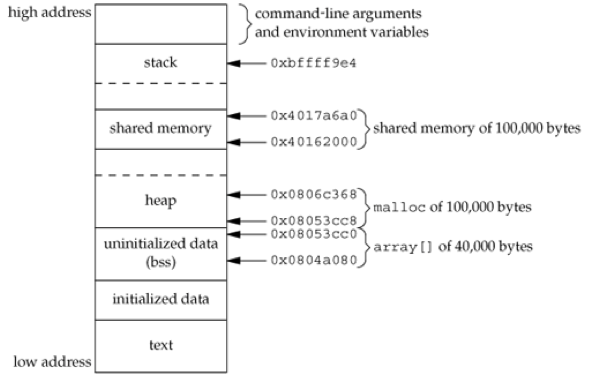
\includegraphics[angle=-90,scale=0.5]{pics/memory-layout.eps}
\end{center}

\subsection{System V IPC: Message Queues}
\begin{itemize}
	\item linked list of messages stored in the kernel
	\item create or open existing queue using {\tt msgget(2)}
	\item add message at end of queue using {\tt msgsnd(2)}
	\item control queue properties using {\tt msgctl(2)}
	\item receive messages from queue using {\tt msgrcv(2)}
\end{itemize}
\vspace{.5in}
The message itself is contained in a user-defined structure such as
\begin{verbatim}
     struct mymsg {
         long mtype;      /* message type */
         char mtext[512]; /* body of message */
     };
\end{verbatim}

\subsection{System V IPC: Message Queues}
\begin{verbatim}
$ cc -Wall msgsend.c -o msgsend
$ cc -Wall msgrecv.c -o msgrecv
$ ipcs -q
$ ./msgsend 1
$ ipcs -q
$ ./msgsend 1
$ ipcs -q
$ ./msgrecv 1
$ ipcs -q
$ ./msgrecv 1
$ ipcs -q
$ ./msgrecv 1
^C
$ ipcs -q
$ ./msgsend 2
$ ipcrm -q <msqid>
\end{verbatim}


\subsection{Sockets: {\tt socketpair(2)}}
\small
\setlength{\unitlength}{1mm}
\begin{center}
	\begin{picture}(150,22)
		\thinlines
		\put(0,0){\framebox(130,22){}}
		\put(10,17){{\tt \#include <sys/socket.h>}}
		\put(10,10){{\tt int socketpair(int {\em d}, int {\em type}, int {\em protocol}, int *{\em sv});}}
	\end{picture}
\end{center}
\Normalsize

The {\tt socketpair(2)} call creates an unnamed pair of connected sockets in
the specified domain {\tt d}, of the specified {\em type}, and using the
optionally specified {\em protocol}.
\\

The descriptors used in referencing the new sockets are returned in {\em
sv[0]} and {\em sv[1]}.  The two sockets are indistinguishable.
\\

{\tt This call is currently implemented only for the UNIX domain.}


\subsection{Sockets: {\tt socketpair(2)}}
\begin{center}
	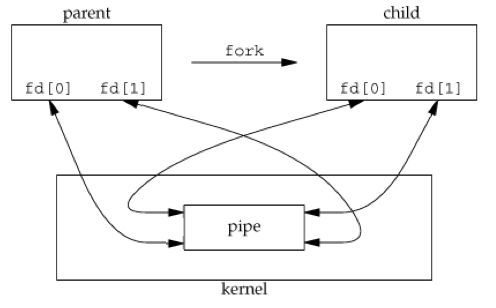
\includegraphics[angle=-90,scale=0.8]{pics/socketpair1.eps}
\end{center}

\subsection{Sockets: {\tt socketpair(2)}}
\begin{center}
	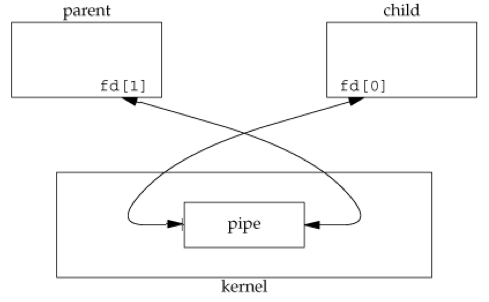
\includegraphics[angle=-90,scale=0.8]{pics/socketpair2.eps}
\end{center}

\subsection{Sockets: {\tt socketpair(2)}}
\begin{verbatim}
$ cc -Wall socketpair.c
$ ./a.out
78482 --> sending: In Xanadu, did Kublai Khan . . .
78483 --> sending: A stately pleasure dome decree . . .
78483 --> reading: In Xanadu, did Kublai Khan . . .
78482 --> reading: A stately pleasure dome decree . . .
$
\end{verbatim}
\vfill
%\hfill \includegraphics[angle=-90,scale=0.9]{pics/j6.eps}


\subsection{Sockets: {\tt socket(2)}}
\small
\setlength{\unitlength}{1mm}
\begin{center}
	\begin{picture}(150,22)
		\thinlines
		\put(0,0){\framebox(130,22){}}
		\put(10,17){{\tt \#include <sys/socket.h>}}
		\put(10,10){{\tt int socket(int {\em domain}, int {\em type}, int {\em protocol});}}
	\end{picture}
\end{center}
\Normalsize
Some of the currently supported domains are:
\\

\small
\begin{tabular}{| l | l |}
	\hline
	{\bf Domain} & {\bf Description} \\
	\hline
	{\tt PF\_LOCAL} 	& 	local (previously UNIX) domain protocols \\
	{\tt PF\_INET}		&	ARPA Internet protocols \\
	{\tt PF\_INET6}		&	ARPA IPv6 (Internet Protocol version 6) protocols \\
	{\tt PF\_ARP}		&	RFC 826 Ethernet Address Resolution Protocol\\
	{\tt ...}		&	...\\
	\hline
\end{tabular}
\Normalsize
\vspace{.5in}

Some of the currently defined types are:
\\

\small
\begin{tabular}{| l | l |}
	\hline
	{\bf Type}		&	{\bf Description} \\
	\hline
	{\tt SOCK\_STREAM}	&	sequenced, reliable, two-way connection based byte streams \\
	{\tt SOCK\_DGRAM}	&	connectionless, unreliable messages of a fixed (typically small)
							maximum length \\
	{\tt SOCK\_RAW}		&	access to internal network protocols and interfaces \\
	{\tt ...}		&	... \\
	\hline
\end{tabular}
\Normalsize

\subsection{Sockets: Datagrams in the UNIX/LOCAL domain}
\begin{verbatim}
1$ cc -Wall udgramsend.c -o send
1$ cc -Wall udgramread.c -o read
1$ ./read
socket --> socket

2$ ls -l socket
srwxr-xr-x  1 jans  users   0 Oct 31 19:17 socket
2$ ./send socket
2$

--> The sea is calm tonight, the tide is full . . .
1$
\end{verbatim}
\vfill
%\hfill \includegraphics[scale=0.9]{pics/j7.eps}


\subsection{Sockets: Datagrams in the UNIX/LOCAL domain}
\begin{itemize}
	\item create socket using {\tt socket(2)}
	\item attach to a socket using {\tt bind(2)}
	\item binding a name in the UNIX domain creates a socket in the file system
	\item both processes need to agree on the name to use
	\item these files are only used for rendezvous, not for message delivery
		once a connection has been established
	\item sockets must be removed using {\tt unlink(2)}
\end{itemize}

\subsection{Sockets: Datagrams in the Internet Domain}
\begin{verbatim}
1$ cc -Wall dgramsend.c -o send
1$ cc -Wall dgramread.c -o read
1$ ./read
Socket has port #64293

2$ netstat -na | grep 64293
udp4       0      0  *.64293                *.*
2$ ./send localhost 64293
2$

--> The sea is calm tonight, the tide is full . . .
1$
\end{verbatim}
\vfill
%\hfill \includegraphics[angle=-90,scale=0.9]{pics/j8.eps}

\subsection{Sockets: Datagrams in the Internet Domain}
\begin{itemize}
	\item Unlike UNIX domain names, Internet socket names are not entered into
		the file system and, therefore, they do not have to be unlinked after the
		socket has been closed.
	\item The local machine address for a socket can be any valid network address
		of the machine, if it has more than one, or it can be the wildcard value
		{\tt INADDR\_ANY}.
	\item ``well-known'' ports (range 1 - 1023) only available to super-user
	\item request any port by calling {\tt bind(2)} with a port number of 0
	\item determine used port number (or other information) using {\tt
		getsockname(2)}
	\item convert between network byteorder and host byteorder using {\tt
		htons(3)} and {\tt ntohs(3)} (which may be noops)
\end{itemize}

\subsection{Sockets: Connections using stream sockets}
\begin{verbatim}
1$ cc -Wall streamread.c -o read
1$ cc -Wall streamwrite.c -o write
1$ ./read
Socket has port #65398

2$ ./write localhost 65398
2$ ./write localhost 65398
--> Half a league, half a league . . .
Ending connection
--> Half a league, half a league . . .
Ending connection

2$ nc localhost 65398
moo
2$
\end{verbatim}
\vfill
%\hfill \includegraphics[angle=-90,scale=0.9]{pics/j9.eps}

\subsection{Sockets: Connections using stream sockets}
\begin{itemize}
	\item connections are asymmetrical:  one process requests a connection,
		the other process accepts the request
	\item one socket is created for each accepted request
	\item mark socket as willing to accept connections using {\tt listen(2)}
	\item pending connections are then {\tt accept(2)}ed
	\item {\tt accept(2)} will block if no connections are available
	\item {\tt select(2)} to check if connection requests are pending
\end{itemize}

XXX add advio select(2) section here?

\subsection{Sockets: Connections using stream sockets}
\begin{verbatim}
1$ cc -Wall strchkread.c -o read
1$ ./read
Socket has port #65398
Do something else
Do something else
2$ ./write localhost 65398
2$ ./write localhost 65398
‐-> Half a league, half a league . . .
Ending connection
Do something else
--> Half a league, half a league . . .
Ending connection
^C
1$
\end{verbatim}
\vfill
%\hfill \includegraphics[angle=-90,scale=0.6]{pics/j10.eps}


\subsection{Sockets: Other Useful Functions}

I/O on sockets is done on descriptors, just like regular I/O, ie the typical
{\tt read(2)} and {\tt write(2)} calls will work.  In order to specify certain
flags, some other functions can be used:

\begin{itemize}
	\item {\tt send(2)}, {\tt sendto(2)} and {\tt sendmsg(2)}
	\item {\tt recv(2)}, {\tt recvfrom(2)} and {\tt recvmsg(2)}
\end{itemize}
To manipulate the options associated with a socket, use {\tt setsockopt(2)}:
\small
\begin{tabular}{| l | l |}
	\hline
	{\bf Option}		&	{\bf Description} \\
	\hline
	{\tt SO\_DEBUG}		&	enables recording of debugging information \\
	{\tt SO\_REUSEADDR}	&	enables local address reuse \\
	{\tt SO\_REUSEPORT}	&	enables duplicate address and port bindings \\
	{\tt SO\_KEEPALIVE}	&	enables keep connections alive\\
	{\tt SO\_DONTROUTE}	&	enables routing bypass for outgoing messages\\
	{\tt SO\_LINGER}	&	linger on close if data present\\
	{\tt SO\_BROADCAST}	&	enables permission to transmit broadcast messages\\
	{\tt SO\_OOBINLINE}	&	enables reception of out-of-band data in band\\
	{\tt SO\_SNDBUF}	&	set buffer size for output\\
	{\tt SO\_RCVBUF}	&	set buffer size for input\\
	{\tt SO\_SNDLOWAT}	&	set minimum count for output\\
	{\tt SO\_RCVLOWAT}	&	set minimum count for input\\
	{\tt SO\_SNDTIMEO}	&	set timeout value for output\\
	{\tt SO\_RCVTIMEO}	&	set timeout value for input\\
	{\tt SO\_TIMESTAMP}	&	enables reception of a timestamp with datagrams\\
	{\tt SO\_TYPE}		&	get the type of the socket (get only)\\
	{\tt SO\_ERROR}		&	get and clear error on the socket (get only)\\
	\hline
\end{tabular}
\Normalsize




\subsection{More Information}
\begin{itemize}
	\item \verb+http://www.cs.stevens.edu/~jschauma/631/ipctut.pdf+
	\item \verb+http://www.cs.stevens.edu/~jschauma/631/ipc.pdf+
	\item \verb+http://www.cs.cf.ac.uk/Dave/C/node25.html+
	\item \verb+http://kohala.com/start/unpv22e/unpv22e.chap12.pdf+
	\item \verb+http://beej.us/guide/bgipc/output/html/singlepage/bgipc.html+
\end{itemize}
\vspace{.5in}

HW\#3: write the basic framework for your final project. \\
\verb+https://www.cs.stevens.edu/~jschauma/631/f16-hw3.html+
%\begin{center}
%\includegraphics[angle=-90,scale=0.75]{pics/nbc.eps}
%\end{center}
%\vspace{\fill}
%\small
%\hfill ...And they call him, Sandy... Clawssss...!

\end{document}
